% Apollo: Person A's part of the two-person, six-minute presentation.
% Keep this file beside the images/ folder when uploading to Prism.
% Compile with pdfLaTeX or XeLaTeX; no installed fonts are required.
% Shared slide 3 has two overlays: click once to change waveform to spectrogram.
\documentclass[aspectratio=169,10pt]{beamer}
\usepackage{graphicx}
\usepackage{array}
\graphicspath{{images/}{docs/presentation/images/}}

\definecolor{ink}{HTML}{16225A}
\definecolor{soft}{HTML}{435071}
\definecolor{teal}{HTML}{00807A}
\definecolor{pale}{HTML}{E9EDF5}
\setbeamercolor{normal text}{fg=ink,bg=white}
\setbeamercolor{frametitle}{fg=ink}
\setbeamerfont{frametitle}{size=\Large,series=\bfseries}
\setbeamertemplate{navigation symbols}{}
\setbeamertemplate{footline}{}
\setbeamersize{text margin left=8mm,text margin right=8mm}
\setbeamertemplate{frametitle}{%
  \vspace*{3mm}\insertframetitle\par
  {\color{teal}\rule{\textwidth}{.6pt}}\vspace{1mm}%
}

% Replace the names before submitting the final shared deck.
\newcommand{\TeamNames}{Presenter A \& Presenter B}
\newcommand{\stagebox}[2]{%
  \colorbox{pale}{\begin{minipage}[c][29mm][c]{26mm}
    \centering{\bfseries\large #1}\par\vspace{2mm}{\small #2}
  \end{minipage}}%
}

\begin{document}

% Shared slide 1: title and problem, 0:00-0:20.
\begin{frame}[plain]
  \vspace*{17mm}
  {\fontsize{34}{38}\selectfont\bfseries Apollo\par}
  \vspace{4mm}
  {\fontsize{18}{22}\selectfont Short audio clip $\longrightarrow$ song title + source time\par}
  \vspace{4mm}
  {\large Noisy recordings, speed edits and covers\par}
  \vfill
  {\bfseries \TeamNames\par}
  {\color{soft}CSE 220 final project \textbar\ September 2026\par}
  \vspace{8mm}
\end{frame}

% Shared slide 2: architecture, 0:45-1:05.
\begin{frame}{How a clip becomes an answer}
  \vspace{6mm}
  \begin{center}
  \begin{tabular}{c@{\hspace{2mm}{\color{teal}\Large$\rightarrow$}\hspace{2mm}}c@{\hspace{2mm}{\color{teal}\Large$\rightarrow$}\hspace{2mm}}c@{\hspace{2mm}{\color{teal}\Large$\rightarrow$}\hspace{2mm}}c}
    \stagebox{Browser}{Mic or tab\\mono WAV} &
    \stagebox{Next.js}{Proxy to\\FastAPI} &
    \stagebox{FastAPI}{Validate; call\\signal code} &
    \stagebox{SQLite}{Find matching\\hashes}
  \end{tabular}
  \end{center}
  \vspace{5mm}
  {\large\bfseries\color{teal}Answer back to the page: song title + where the clip begins}
  \vspace{3mm}

  {\color{soft}Signal code builds fingerprints; SQLite searches an indexed catalog.}
\end{frame}

% Shared slide 3, overlay 1: capture and standardize.
\begin{frame}{From sound to spectrogram}
\only<1>{%
  {\bfseries\color{teal}1 / 2\quad Capture the waveform}\hfill
  {\color{soft}time $\rightarrow$; height = signal amplitude}\par\vspace{2mm}
  \centering
  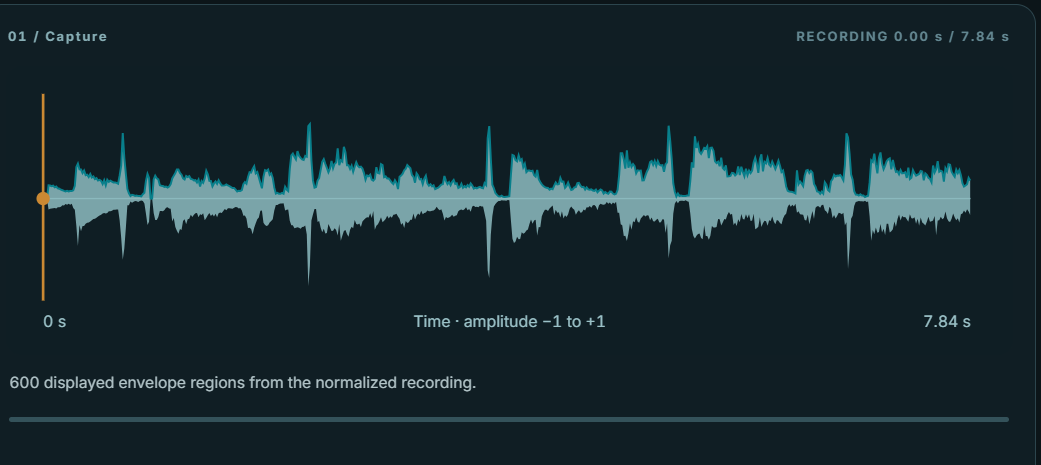
\includegraphics[height=5.45cm]{capture.png}\par\vspace{2mm}
  {\small Mono + peak normalization + 22,050 samples/second for both song and query.}
}
\only<2>{%
  {\bfseries\color{teal}2 / 2\quad STFT makes a frequency map}\hfill
  {\color{soft}time $\rightarrow$, frequency $\uparrow$}\par\vspace{2mm}
  \centering
  % Crop the original screenshot to its graph; the explanatory side panel is excluded.
  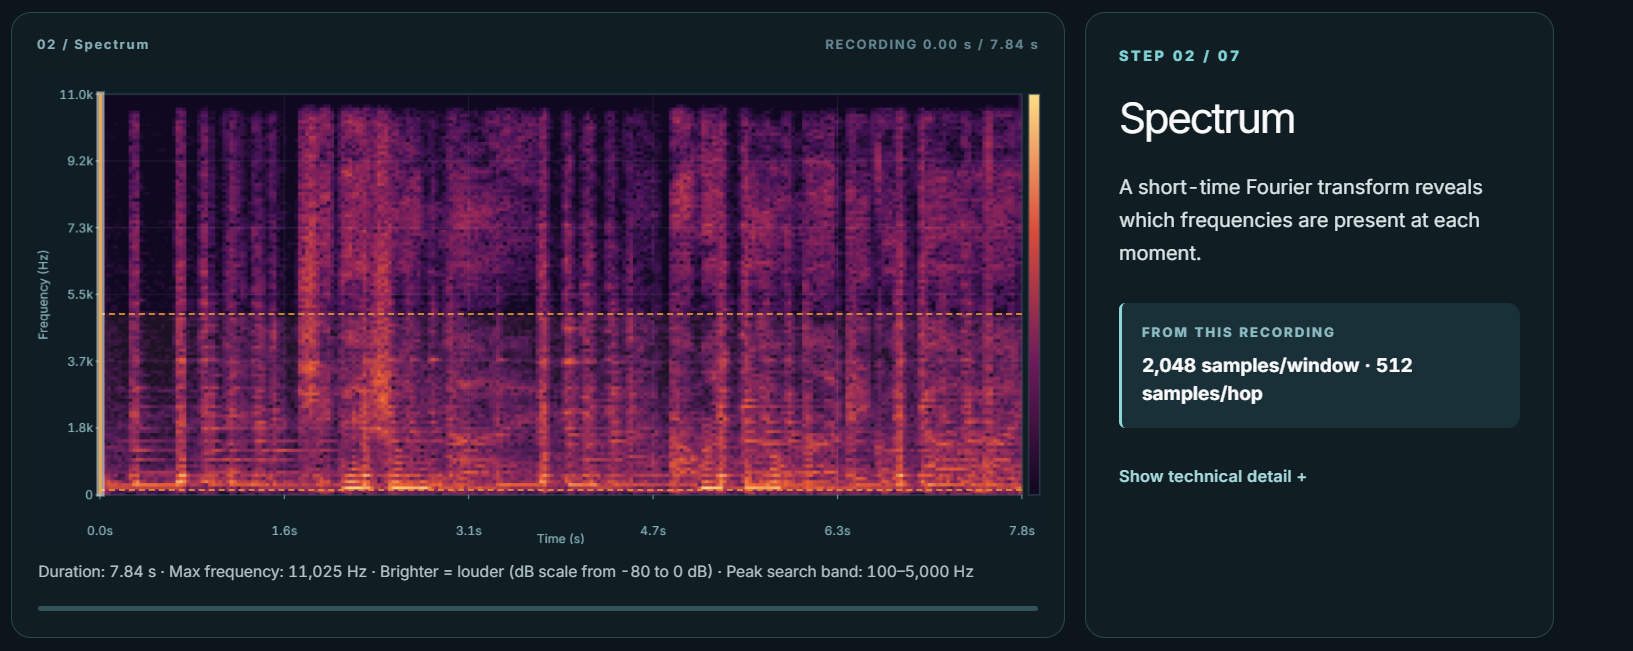
\includegraphics[height=5.45cm,trim=21bp 64bp 356bp 44bp,clip]{spectrum.png}\par\vspace{2mm}
  {\small 2,048-sample windows (93 ms); hop 512 (23 ms). Each window gives one column.}
}
\end{frame}

% Shared slide 4: real peak map, 1:40-2:00.
\begin{frame}[t]{Keep strong local peaks}
  \begin{center}
  {\bfseries\color{teal}Each dot marks one frequency at one moment.}\par\vspace{2mm}
  % Crop the graph-only screenshot to its plotted area and axes.
  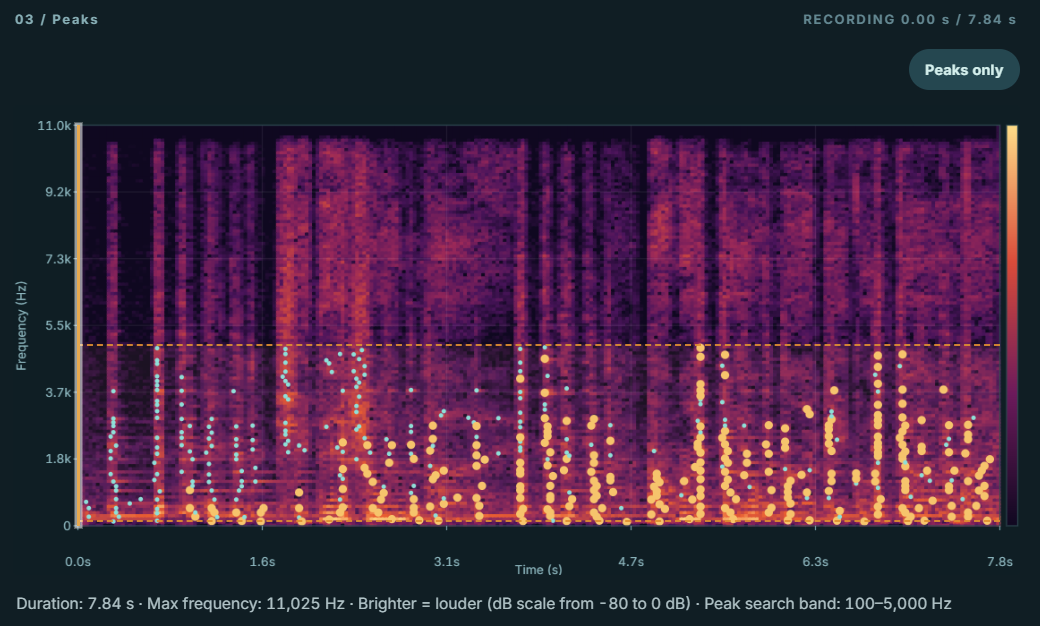
\includegraphics[height=5.2cm,trim=6bp 58bp 12bp 66bp,clip]{peaks.png}\par\vspace{2mm}
  {\small 15 frequency bins $\times$ 9 time frames \quad $\cdot$ \quad 100--5,000 Hz; $\geq -60$ dB
    \quad $\cdot$ \quad at most 60 peaks/second}
  \end{center}
\end{frame}

% Shared slide 6: speed search, 3:15-3:25.
\begin{frame}{How Apollo handles edited audio}
  \vspace{4mm}
  \renewcommand{\arraystretch}{1.8}
  \begin{center}
  \begin{tabular}{>{\bfseries}lcc}
    & Frequency / pitch & Time between peaks\\\hline
    Speed edit & changes & changes\\
    Pitch-only edit & changes & stays the same
  \end{tabular}
  \end{center}
  \vspace{5mm}
  {\large\bfseries\color{teal}78 quick guesses: 39 speed + 39 pitch-only factors}
  \vspace{3mm}

  {\large Rescale detected peaks $\rightarrow$ make new fingerprints $\rightarrow$ test the best guesses.}
  \vspace{3mm}

  {\color{soft}This fallback runs when ordinary fingerprint matching misses an edit.}
\end{frame}

\end{document}
